\documentclass[a4paper, 10pt]{scrartcl}\usepackage[]{graphicx}\usepackage[]{color}
%% maxwidth is the original width if it is less than linewidth
%% otherwise use linewidth (to make sure the graphics do not exceed the margin)
\makeatletter
\def\maxwidth{ %
  \ifdim\Gin@nat@width>\linewidth
    \linewidth
  \else
    \Gin@nat@width
  \fi
}
\makeatother

\definecolor{fgcolor}{rgb}{0.345, 0.345, 0.345}
\newcommand{\hlnum}[1]{\textcolor[rgb]{0.686,0.059,0.569}{#1}}%
\newcommand{\hlstr}[1]{\textcolor[rgb]{0.192,0.494,0.8}{#1}}%
\newcommand{\hlcom}[1]{\textcolor[rgb]{0.678,0.584,0.686}{\textit{#1}}}%
\newcommand{\hlopt}[1]{\textcolor[rgb]{0,0,0}{#1}}%
\newcommand{\hlstd}[1]{\textcolor[rgb]{0.345,0.345,0.345}{#1}}%
\newcommand{\hlkwa}[1]{\textcolor[rgb]{0.161,0.373,0.58}{\textbf{#1}}}%
\newcommand{\hlkwb}[1]{\textcolor[rgb]{0.69,0.353,0.396}{#1}}%
\newcommand{\hlkwc}[1]{\textcolor[rgb]{0.333,0.667,0.333}{#1}}%
\newcommand{\hlkwd}[1]{\textcolor[rgb]{0.737,0.353,0.396}{\textbf{#1}}}%
\let\hlipl\hlkwb

\usepackage{framed}
\makeatletter
\newenvironment{kframe}{%
 \def\at@end@of@kframe{}%
 \ifinner\ifhmode%
  \def\at@end@of@kframe{\end{minipage}}%
  \begin{minipage}{\columnwidth}%
 \fi\fi%
 \def\FrameCommand##1{\hskip\@totalleftmargin \hskip-\fboxsep
 \colorbox{shadecolor}{##1}\hskip-\fboxsep
     % There is no \\@totalrightmargin, so:
     \hskip-\linewidth \hskip-\@totalleftmargin \hskip\columnwidth}%
 \MakeFramed {\advance\hsize-\width
   \@totalleftmargin\z@ \linewidth\hsize
   \@setminipage}}%
 {\par\unskip\endMakeFramed%
 \at@end@of@kframe}
\makeatother

\definecolor{shadecolor}{rgb}{.97, .97, .97}
\definecolor{messagecolor}{rgb}{0, 0, 0}
\definecolor{warningcolor}{rgb}{1, 0, 1}
\definecolor{errorcolor}{rgb}{1, 0, 0}
\newenvironment{knitrout}{}{} % an empty environment to be redefined in TeX

\usepackage{alltt}  %livre

% Permet l'encodage avec le Unicode Transformation Format-8-bit
\usepackage[utf8]{inputenc}
% Permet la gestion des caractères accentués ainsi que la stabilité des impressions en P.D.F.
\usepackage[T1]{fontenc}
% Permet la stabilisation de l'écriture
\usepackage{lmodern, textcomp}
% Permet d'utiliser les liens hypertexte sans altérer la bibliothèque KOMA
\usepackage{scrhack}
\KOMAoptions{hyperref=false}
% Utilise les règles gramaticales françaises
\usepackage[french]{babel}

%Utilise les règles typographique de la bibliothéques KOMA
\setkomafont{author}{\scshape}
%\usepackage{blindtext}

% Package pour avoir plus d'arguments dans ses commandes.
\usepackage{xargs}
%Package pour plus de souplesse
\usepackage{tabularx}

%Package pour les listes indexées
\usepackage{enumitem}

%Bibliothèque mathématiques pour la police.
\usepackage{amsfonts}
%Bibliothèques mathématiques générale.
\usepackage{amsmath}
\usepackage{amssymb}
%Pour appliquer \mathbb à des nombres
\usepackage{bbm}
%Package pour l'indexation de matrices
\usepackage{blkarray}
%\usepackage{dsfont}
%Package pour spreadsheet
\usepackage{spreadtab}
\usepackage{fp}
\usepackage{xstring}
\renewcommand\STprintnum[1]{\numprint{#1}}
\STsetdecimalsep{,}
\STautoround{6}
\usepackage{eurosym}
%Bibliothèque pour l'affichage de nombre avec la typographie définie
\usepackage{numprint}
\newcommand{\np}[1]{\numprint{#1}}
% Pour la notation scientifique
\usepackage{siunitx}
\sisetup{locale= FR,exponent-product=., unit-mode = text}
\DeclareSIUnit\year{ann\'{e}ee}
%Positionnement des images
\usepackage{float}
\usepackage{subcaption}
%Utilisation des couleurs
\usepackage{xcolor}
% Package pour le soulignement
\usepackage{color,soulutf8}
\setulcolor{red}
% Package pour les annotations
\usepackage{todonotes}
%\usepackage[pygments]{pythontex} % Pour utiliser Python
%\usepackage{fvextra} % Utile pour la mise en forme du code source inséré
%Package pour la programmation
\usepackage{listings}
% Package pour les scripts en R
\lstset{language=R,
    basicstyle=\small\ttfamily,
    stringstyle=\color{DarkGreen},
    otherkeywords={0,1,2,3,4,5,6,7,8,9},
    morekeywords={TRUE,FALSE},
    deletekeywords={data,frame,length,as,character},
    keywordstyle=\color{blue},
    commentstyle=\color{DarkGreen},
    }

%Définition de couleurs:
\definecolor{bleudefrance}{rgb}{.19, .55, .91}
\definecolor{pakistangreen}{rgb}{.0, .4, .0}
\definecolor{rossocorsa}{rgb}{0.83, 0.0, 0.0}
\definecolor{persimmon}{rgb}{0.93, 0.35, 0.0}
\definecolor{bronze}{rgb}{0.8, 0.5, 0.2}
% Annotation auteur
\newcommand{\Moi}[1]{\todo[color = teal!40]{#1}}
\newcommand{\Cnsl}[1]{\todo[color = pakistangreen!40]{#1}}
\newcommand{\MeG}[1]{\todo[color = rossocorsa!40]{#1}}
%Notation récurrante:
\newcommandx{\hb}[1]{\widehat{\beta_{#1}}}
\newcommandx{\prth}[4]{\left( #1_{#2} \right)_{#3\leq #2 \leq #4}}
% Encadrement des résultats
\newcommand{\enc}[1]{\fcolorbox{rossocorsa}{white}{#1}}
\newcommand{\encB}[1]{\fcolorbox{bleudefrance}{white}{#1}}
\newcommand{\encV}[1]{\fcolorbox{pakistangreen}{white}{#1}}
\newcommand{\encN}[1]{\fcolorbox{black}{white}{#1}}
% Soulignement couleur
\newcommandx{\sN}[1]{\setulcolor{black}\ul{#1}}
\newcommandx{\sR}[1]{\setulcolor{rossocorsa}\ul{#1}}
\newcommandx{\sB}[1]{\setulcolor{bleudefrance}\ul{#1}}
\newcommandx{\sV}[1]{\setulcolor{pakistangreen}\ul{#1}}
\newcommandx{\sT}[1]{\setulcolor{teal}\ul{#1}}
\newcommandx{\sO}[1]{\setulcolor{persimmon}\ul{#1}}
\newcommandx{\sG}[1]{\setulcolor{tiger}\ul{#1}}
% Text de couleur
\newcommandx{\tR}[1]{\textcolor{rossocorsa}{#1}}
\newcommandx{\tB}[1]{\textcolor{bleudefrance}{#1}}
\newcommandx{\tV}[1]{\textcolor{pakistangreen}{#1}}
\newcommandx{\tT}[1]{\textcolor{teal}{#1}}
\newcommandx{\tO}[1]{\textcolor{persimmon}{#1}}
\newcommandx{\tBr}[1]{\textcolor{bronze}{#1}}
% Écriture intervalle
\newcommandx{\inter}[2]{\left[\![#1, #2]\!\right]}
% Écriture intégrale
\newcommandx{\Su}[2]{{\displaystyle \int_{#1}^{#2}}}
% Écriture somme sigma
\newcommandx{\su}[2]{{\displaystyle \sum_{#1}^{#2}}}
% Écriture produit pi
\newcommandx{\prd}[2]{{\displaystyle \prod_{#1}^{#2}}}
%Écriture limite lim
\newcommandx{\lm}[2]{{\displaystyle \lim_{#1\to #2}}}
% Écriture P(X)
\newcommandx{\prob}[1]{\mathbb{P}\left(#1\right)}
% Écriture P_{\{Y\}}({X})
\newcommandx{\probC}[2]{\mathbb{P}_{#1}\left(#2\right)}
% Écriture P({X})
\newcommandx{\Prob}[1]{\mathbb{P}\left(\left\{#1 \right\}\right)}
% Écriture P_{\{Y\}}({X})
\newcommandx{\ProbC}[2]{\mathbb{P}_{\left\{#1\right\}}\left(\left\{#2\right\}\right)}
% Ecriture Esperance et Variance
\newcommandx{\E}[1]{\mathbb{E}\left(#1\right)}
\newcommandx{\Ec}[2]{\mathbb{E}_{\left\{#1\right\}}\left(#2\right)}
\newcommandx{\V}[1]{\mathbb{V}\left(#1\right)}
\newcommandx{\Vc}[2]{\mathbb{V}_{\left\{#1\right\}}\left(#2\right)}
%Symbole de la norme
\newcommandx{\norm}[1]{\left\lVert#1\right\rVert}

\title{Summarise Course/Methods}
\author{Siger}
\IfFileExists{upquote.sty}{\usepackage{upquote}}{}
\begin{document}

\maketitle

Si Dieu est infini, alors je suis une partie de Dieu sinon je serai sa limite\ldots

\tableofcontents

\section{Conceptual}
\subsection{1)}
\begin{figure}[H]
	\begin{center}
		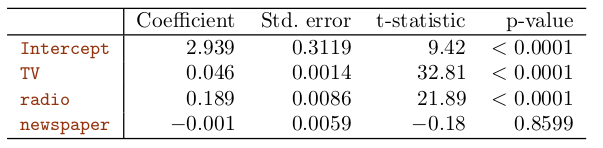
\includegraphics[width=\textwidth]{./images/table3_4.png}
	\end{center}
	\caption{Analyse p-value}
	\label{fig:1}
\end{figure}
Noting $H_{0_{variable}}$ the null hypotheses to which the p-values 
correspond then for $variable\in\left\{ TV,radio,newspaper \right\}$
$H_{0}$ is true if and only if there is no relationship between $sales\text{ and }variable$.\\
Regarding $p-values$ of $intercept, TV, radio$ we observe that it is
unlikely to observe such a 
substantial association between each of these variables and $sales$ due to chance.\\
Then we can infer that it exists a association between each of these 
variables and $sales$, unlike $newspaper$.
\subsection{2.}
K-Nearest neighbors classifier: attempts to estimate the conditional
distribution of $Y$ given $X$, and then classify a
given observation to the class with highest estimated probability.
\begin{center}
	$\ProbC{X=x_{0}}{Y=j}=\dfrac{1}{K}\su{ {i\in\mathcal{N}_{0}}}{}I(y_{i}=j)$
\end{center}

K-Nearest neighbors regression: given a value for $K$ and a prediction 
point $x_{0}$ , KNN regression first identifies the $K$ training 
observations that are closest to
$x_{0}$ , represented by $\mathcal{N}_{0}$ . It then estimates $f(x_{0})$ using the
average of all the training responses in $\mathcal{N}_{0}$
\begin{center}
	$\hat{f}(x_{0})=\dfrac{1}{K}\su{ {x_{i}\in\mathcal{N}_{0}}}{}y_{i}$
\end{center}
\subsection{3.}
Fait sur papier
\subsection{4.}
For a linear regression without intercept we have the ith fitted value
in the form: $\hat{y}_{i}=x_{i}\hat{\beta}\text{ with }\hat{\beta}=
\dfrac{\su{ {i=1}}{n}x_{i}y_{i}}{\su{ {i=1}}{n}x_{i}^{2}}$\\Then we get
$\hat{y_{i}}=\su{ {i=1}}{n}\dfrac{x_{i}}{\su{ {i=1}}{n}x_{i}^{2}}y_{i}=
\su{ {i=1}}{n}a_{i}y_{i}$
``We interpret this result by saying that the fitted values from
linear regression are linear combinations of the response values.''
\subsection{6.}
$\hat{y_{i}}=\hat{\beta_{0}}+\hat{\beta_{1}}x_{i}\text{ but }\beta_{0}=
\overline{y}-\beta_{1}\overline{x}\text{ then }\hat{y_{i}}=\overline{y}
-\beta_{1}\overline{x}+\beta_{1}x_{i}$\\ For $x_{i}=\overline{x}$ we
get $\hat{y_{i}}=\overline{y}$, so the point $(\overline{x},\overline{y})$ belongs to the least square line.
\subsection{7.}

\section{Applied}
\subsection{8.}
\begin{abstract}
\begin{knitrout}
\definecolor{shadecolor}{rgb}{0.969, 0.969, 0.969}\color{fgcolor}\begin{kframe}
\begin{alltt}
\hlkwd{library}\hlstd{(MASS)}
\hlkwd{library}\hlstd{(ISLR)}
\hlstd{autoDF}\hlkwb{=}\hlstd{Auto}
\hlstd{lm.fit} \hlkwb{=} \hlkwd{lm}\hlstd{(mpg}\hlopt{~}\hlstd{horsepower,} \hlkwc{data}\hlstd{=autoDF)} \hlcom{#simple linear regression horsepower onto mpg}
\hlkwd{summary}\hlstd{(lm.fit)} \hlcom{#Displaying global information}
\end{alltt}
\begin{verbatim}
## 
## Call:
## lm(formula = mpg ~ horsepower, data = autoDF)
## 
## Residuals:
##      Min       1Q   Median       3Q      Max 
## -13.5710  -3.2592  -0.3435   2.7630  16.9240 
## 
## Coefficients:
##              Estimate Std. Error t value Pr(>|t|)    
## (Intercept) 39.935861   0.717499   55.66   <2e-16 ***
## horsepower  -0.157845   0.006446  -24.49   <2e-16 ***
## ---
## Signif. codes:  0 '***' 0.001 '**' 0.01 '*' 0.05 '.' 0.1 ' ' 1
## 
## Residual standard error: 4.906 on 390 degrees of freedom
## Multiple R-squared:  0.6059,	Adjusted R-squared:  0.6049 
## F-statistic: 599.7 on 1 and 390 DF,  p-value: < 2.2e-16
\end{verbatim}
\end{kframe}
\end{knitrout}
\end{abstract}
\begin{itemize}
	\item[i] Regarding the p-value, it seems there is a 
		relationship between predictor and the response
	\item[ii] This relationship is weak because  
		$\widehat{horsepower}=-0.157845$
	\item[iii] The relationship is negative because $-0.157845<0$
	\item[iv] The predicted mpg associated with a horsepower 
		of 98 is
		\begin{abstract}
\begin{knitrout}
\definecolor{shadecolor}{rgb}{0.969, 0.969, 0.969}\color{fgcolor}\begin{kframe}
\begin{alltt}
\hlkwd{coef}\hlstd{(lm.fit)[}\hlnum{1}\hlstd{]} \hlopt{+} \hlkwd{coef}\hlstd{(lm.fit)[}\hlnum{2}\hlstd{]}\hlopt{*}\hlnum{98}
\end{alltt}
\begin{verbatim}
## (Intercept) 
##    24.46708
\end{verbatim}
\end{kframe}
\end{knitrout}
		\end{abstract}
		And confidence and prediction interval, for 
		$horsepower=98$ are respectively:
		\begin{abstract}
\begin{knitrout}
\definecolor{shadecolor}{rgb}{0.969, 0.969, 0.969}\color{fgcolor}\begin{kframe}
\begin{alltt}
\hlkwd{predict}\hlstd{(lm.fit,} \hlkwd{data.frame}\hlstd{(}\hlkwc{horsepower}\hlstd{=}\hlnum{98}\hlstd{),} \hlkwc{interval}\hlstd{=}\hlstr{"confidence"}\hlstd{)}
\end{alltt}
\begin{verbatim}
##        fit      lwr      upr
## 1 24.46708 23.97308 24.96108
\end{verbatim}
\begin{alltt}
\hlkwd{predict}\hlstd{(lm.fit,} \hlkwd{data.frame}\hlstd{(}\hlkwc{horsepower}\hlstd{=}\hlnum{98}\hlstd{),} \hlkwc{interval}\hlstd{=}\hlstr{"prediction"}\hlstd{)}
\end{alltt}
\begin{verbatim}
##        fit     lwr      upr
## 1 24.46708 14.8094 34.12476
\end{verbatim}
\end{kframe}
\end{knitrout}
		\end{abstract}
\end{itemize}
\paragraph{(b)}
Plot of the response and the predictor:
\begin{abstract}
\begin{knitrout}
\definecolor{shadecolor}{rgb}{0.969, 0.969, 0.969}\color{fgcolor}\begin{kframe}
\begin{alltt}
\hlkwd{attach}\hlstd{(Auto)}
\hlkwd{plot}\hlstd{(horsepower, mpg,} \hlkwc{col}\hlstd{=}\hlstr{'red'}\hlstd{,} \hlkwc{pch}\hlstd{=}\hlstr{'+'}\hlstd{)}
\hlkwd{abline}\hlstd{(lm.fit,} \hlkwc{lwd}\hlstd{=}\hlnum{3}\hlstd{,} \hlkwc{col}\hlstd{=}\hlstr{'green'}\hlstd{)}
\end{alltt}
\end{kframe}
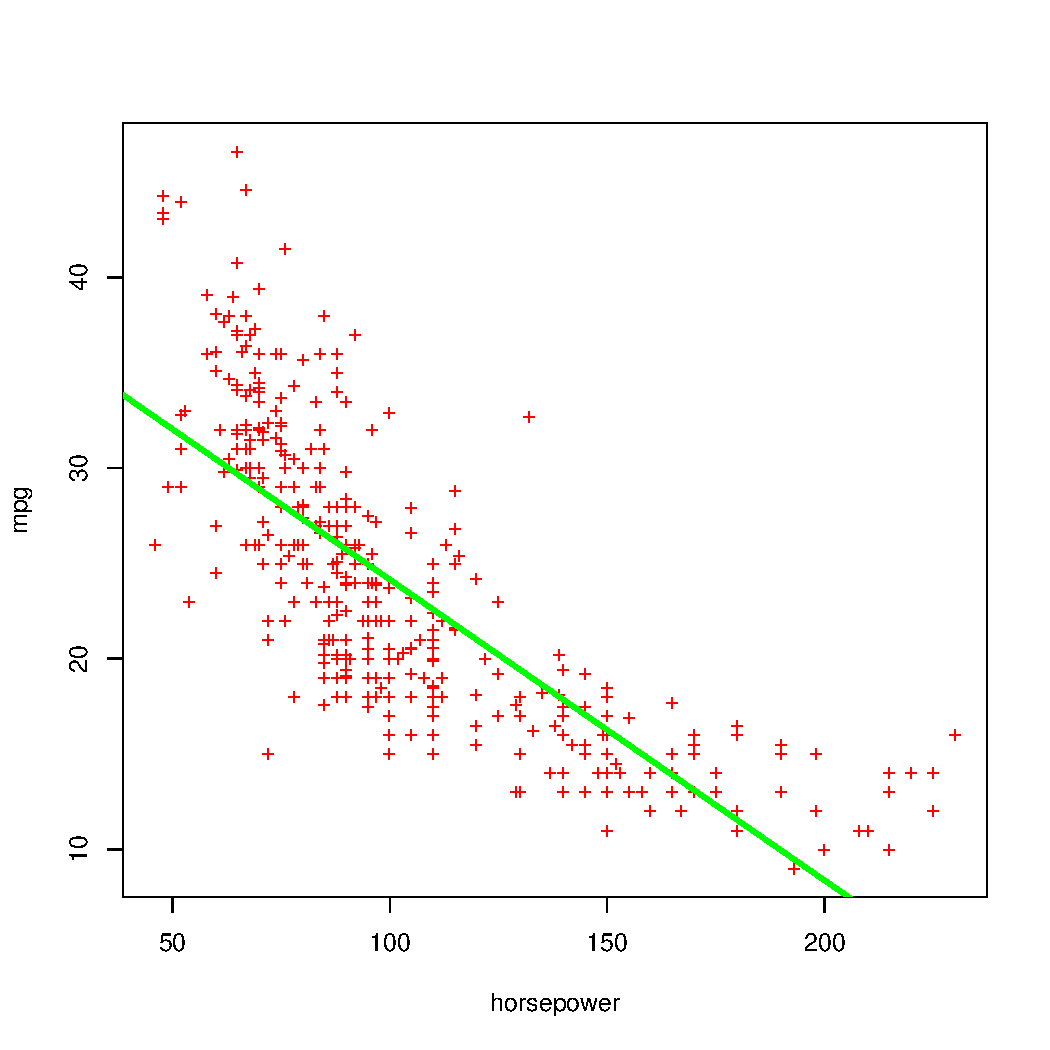
\includegraphics[width=\maxwidth]{figure/unnamed-chunk-4-1} 

\end{knitrout}
\end{abstract}
\paragraph{(c)}
Plot of the response and the predictor:
\begin{abstract}
\begin{knitrout}
\definecolor{shadecolor}{rgb}{0.969, 0.969, 0.969}\color{fgcolor}\begin{kframe}
\begin{alltt}
\hlkwd{par}\hlstd{(}\hlkwc{mfrow}\hlstd{=}\hlkwd{c}\hlstd{(}\hlnum{2}\hlstd{,}\hlnum{2}\hlstd{))}
\hlkwd{plot}\hlstd{(lm.fit)}
\end{alltt}
\end{kframe}
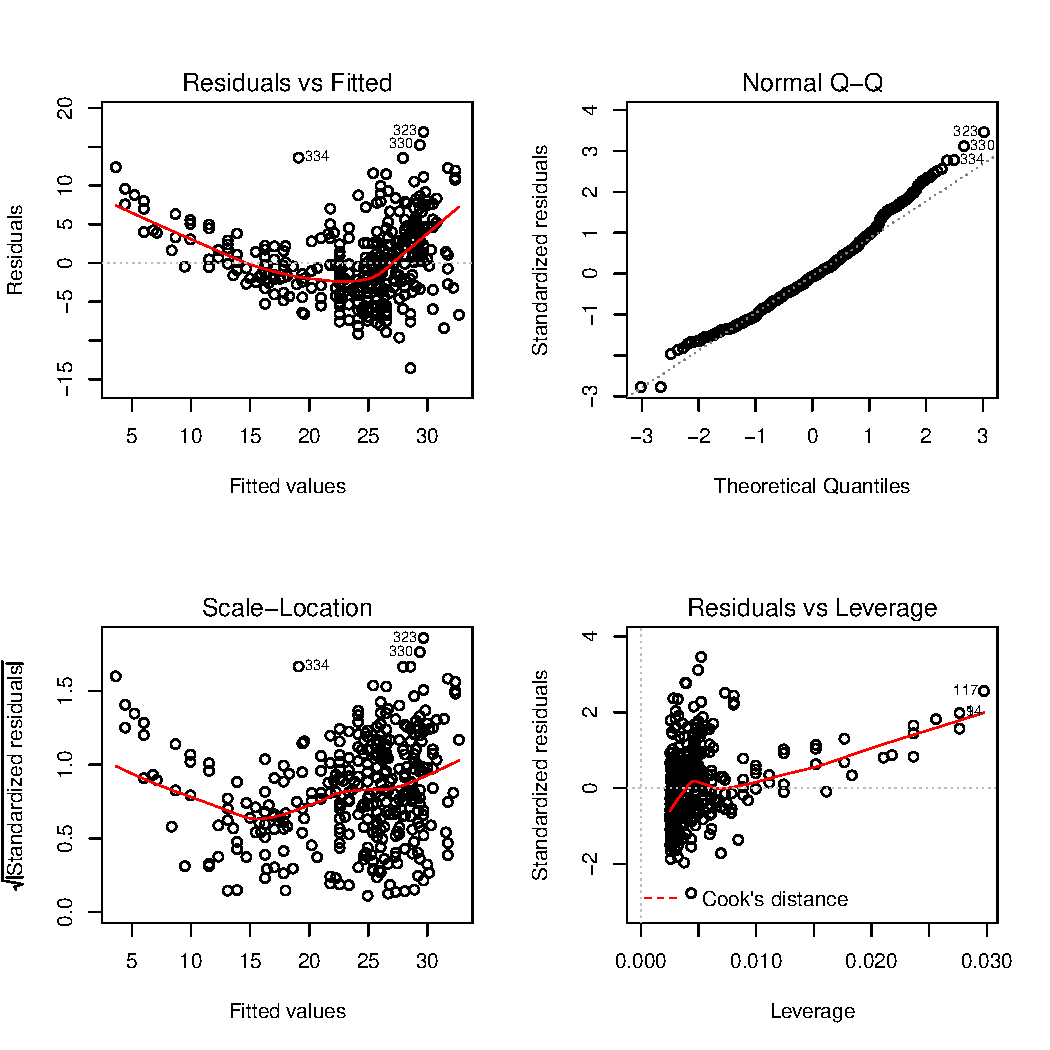
\includegraphics[width=\maxwidth]{figure/unnamed-chunk-5-1} 

\end{knitrout}
\end{abstract}
Regarding plots above, the first ``Residuals vs Fitted'' plots shows us
that the linear model is not a very suitable model for these data.\\
And the ``Normal Q-Q'' shows us that residuals or not normally 
spread.\\ Then the ``Scale-Location'' shows us that residuals are not 
equally spread along the range of predictors, so the equal variance
(homoscedasticity) is not adapted to these data.\\
Finally the ``Residuals vs Leverage'' shows us that it is not seems to
exist very big outliers.
\subsection{9}
\paragraph{(a)} Scatterplot matrix which including all of the variables
in the data set
\begin{abstract}
\begin{knitrout}
\definecolor{shadecolor}{rgb}{0.969, 0.969, 0.969}\color{fgcolor}\begin{kframe}
\begin{alltt}
\hlkwd{pairs}\hlstd{(Auto)}
\end{alltt}
\end{kframe}
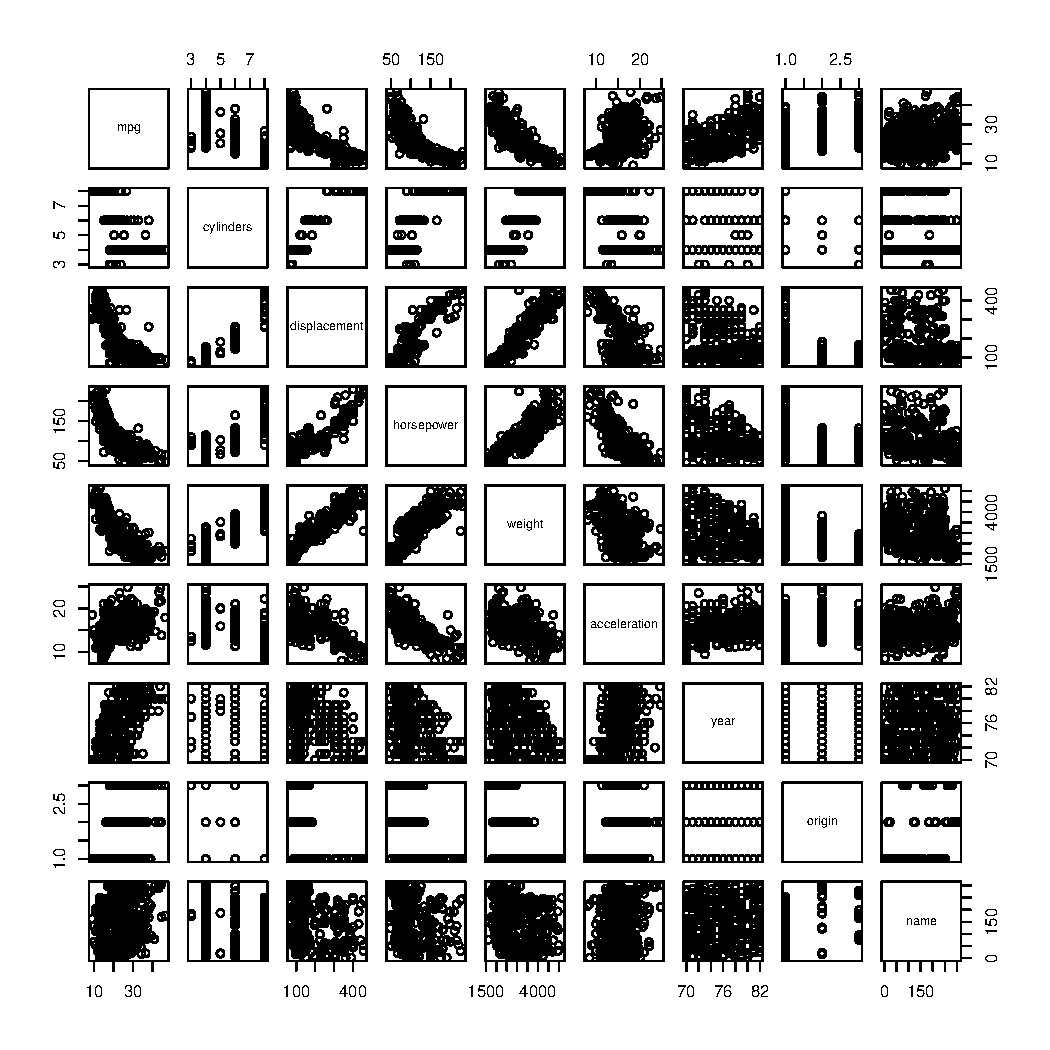
\includegraphics[width=\maxwidth]{figure/unnamed-chunk-6-1} 

\end{knitrout}
\end{abstract}
\paragraph{(b)}The matrix of correlations between the variables, and
we have excluded then ``name'' variable:
\begin{abstract}
\begin{knitrout}
\definecolor{shadecolor}{rgb}{0.969, 0.969, 0.969}\color{fgcolor}\begin{kframe}
\begin{alltt}
\hlstd{Table} \hlkwb{=} \hlkwd{data.frame}\hlstd{(Auto)}
\hlkwd{cor}\hlstd{(Table[,} \hlopt{-}\hlnum{9}\hlstd{])}
\end{alltt}
\begin{verbatim}
##                     mpg  cylinders displacement horsepower     weight
## mpg           1.0000000 -0.7776175   -0.8051269 -0.7784268 -0.8322442
## cylinders    -0.7776175  1.0000000    0.9508233  0.8429834  0.8975273
## displacement -0.8051269  0.9508233    1.0000000  0.8972570  0.9329944
## horsepower   -0.7784268  0.8429834    0.8972570  1.0000000  0.8645377
## weight       -0.8322442  0.8975273    0.9329944  0.8645377  1.0000000
## acceleration  0.4233285 -0.5046834   -0.5438005 -0.6891955 -0.4168392
## year          0.5805410 -0.3456474   -0.3698552 -0.4163615 -0.3091199
## origin        0.5652088 -0.5689316   -0.6145351 -0.4551715 -0.5850054
##              acceleration       year     origin
## mpg             0.4233285  0.5805410  0.5652088
## cylinders      -0.5046834 -0.3456474 -0.5689316
## displacement   -0.5438005 -0.3698552 -0.6145351
## horsepower     -0.6891955 -0.4163615 -0.4551715
## weight         -0.4168392 -0.3091199 -0.5850054
## acceleration    1.0000000  0.2903161  0.2127458
## year            0.2903161  1.0000000  0.1815277
## origin          0.2127458  0.1815277  1.0000000
\end{verbatim}
\end{kframe}
\end{knitrout}
\end{abstract}
\paragraph{(c)} We perform a multiple linear regression with mpg as the
response and all other variables except name as the predictors.
\begin{abstract}
\begin{knitrout}
\definecolor{shadecolor}{rgb}{0.969, 0.969, 0.969}\color{fgcolor}\begin{kframe}
\begin{alltt}
\hlstd{lm.fit} \hlkwb{=} \hlkwd{lm}\hlstd{(mpg}\hlopt{~}\hlstd{.}\hlopt{-}\hlstd{name,} \hlkwc{data}\hlstd{=Auto)}
\hlkwd{summary}\hlstd{(lm.fit)}
\end{alltt}
\begin{verbatim}
## 
## Call:
## lm(formula = mpg ~ . - name, data = Auto)
## 
## Residuals:
##     Min      1Q  Median      3Q     Max 
## -9.5903 -2.1565 -0.1169  1.8690 13.0604 
## 
## Coefficients:
##                Estimate Std. Error t value Pr(>|t|)    
## (Intercept)  -17.218435   4.644294  -3.707  0.00024 ***
## cylinders     -0.493376   0.323282  -1.526  0.12780    
## displacement   0.019896   0.007515   2.647  0.00844 ** 
## horsepower    -0.016951   0.013787  -1.230  0.21963    
## weight        -0.006474   0.000652  -9.929  < 2e-16 ***
## acceleration   0.080576   0.098845   0.815  0.41548    
## year           0.750773   0.050973  14.729  < 2e-16 ***
## origin         1.426141   0.278136   5.127 4.67e-07 ***
## ---
## Signif. codes:  0 '***' 0.001 '**' 0.01 '*' 0.05 '.' 0.1 ' ' 1
## 
## Residual standard error: 3.328 on 384 degrees of freedom
## Multiple R-squared:  0.8215,	Adjusted R-squared:  0.8182 
## F-statistic: 252.4 on 7 and 384 DF,  p-value: < 2.2e-16
\end{verbatim}
\end{kframe}
\end{knitrout}
\end{abstract}
\subparagraph{i.} The predictors displacement, horsepower, and weight
do not seem to have a relationship with the response.
\subparagraph{ii.} It seems that there is a relationship is statically
significant between the response and the following predictors: origin,
year, weight and in lesser measure displacement.
\subparagraph{iii.} The coefficient for the year variable suggests that
an increasing of 10 years, bring on average 75 miles per gallon to a
car.
\paragraph{(d)} We produce diagnostic plots of the linear regression 
fit:
\begin{abstract}
\begin{knitrout}
\definecolor{shadecolor}{rgb}{0.969, 0.969, 0.969}\color{fgcolor}\begin{kframe}
\begin{alltt}
\hlstd{lm.fit} \hlkwb{=} \hlkwd{lm}\hlstd{(mpg}\hlopt{~}\hlstd{.}\hlopt{-}\hlstd{name,} \hlkwc{data}\hlstd{=Auto)}
\hlkwd{par}\hlstd{(}\hlkwc{mfrow}\hlstd{=}\hlkwd{c}\hlstd{(}\hlnum{2}\hlstd{,}\hlnum{2}\hlstd{))}
\hlkwd{plot}\hlstd{(lm.fit)}
\end{alltt}
\end{kframe}
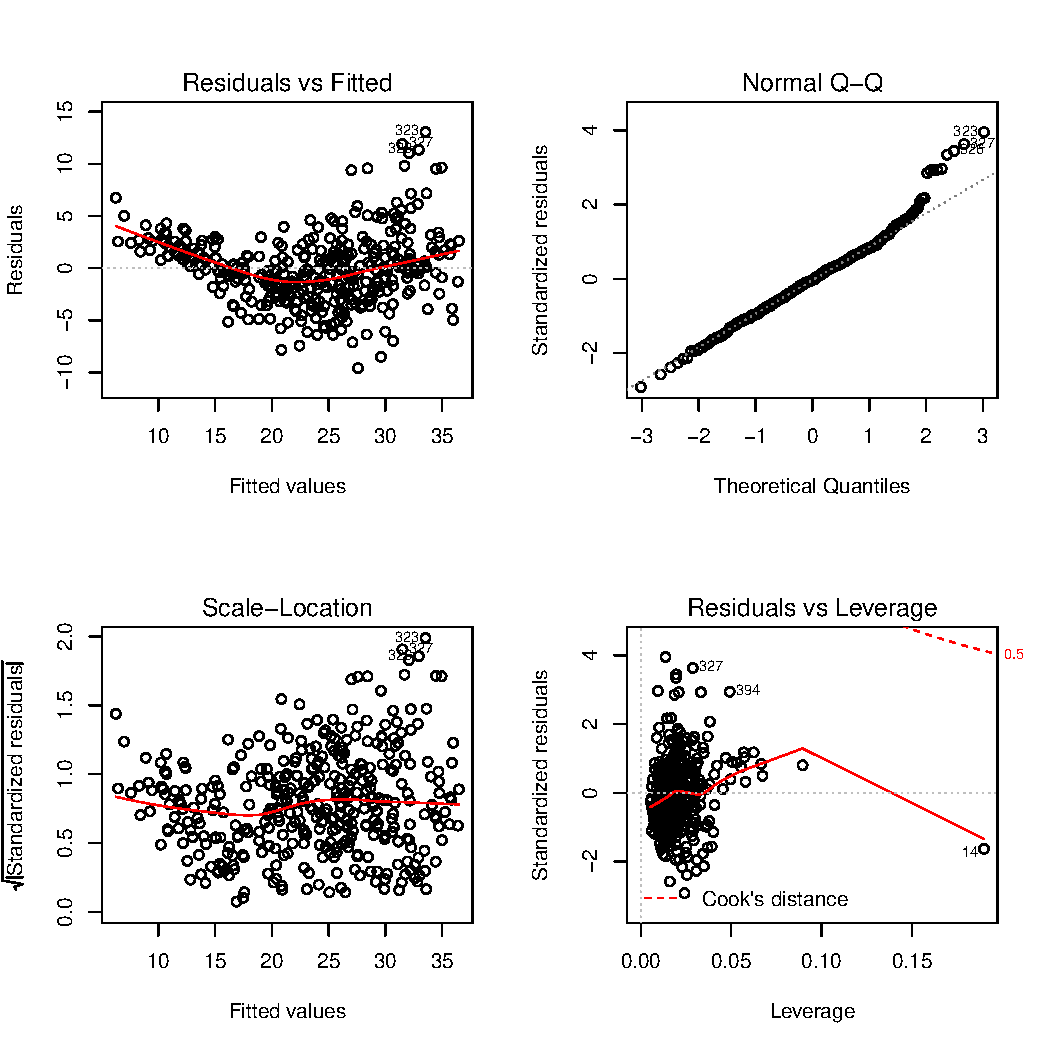
\includegraphics[width=\maxwidth]{figure/unnamed-chunk-9-1} 

\end{knitrout}
\end{abstract}
The ``Residuals vs Fitted'' plot shows us that relationship is not 
really linear.\\ And the ``Normal Q-Q'' plot shows that the very most
part of residuals are normally spread.\\ Then the ``Scale-Location''
shows us that the homoscedasticity assumption is enough respected.\\
Finally the ``Residuals vs Leverage'' shows us that there is not 
significant of outliers.
\end{document}
